\documentclass{standalone}

\usepackage{tikz}
\usetikzlibrary{calc}

\begin{document}
% CBC-mode encryption.
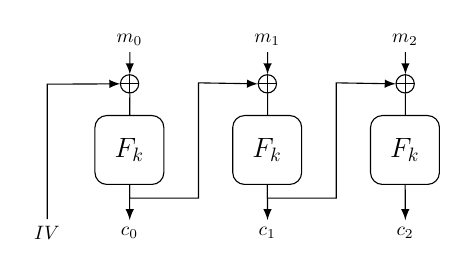
\begin{tikzpicture}[scale=0.7, every node/.style={scale=0.7}]
\foreach \x in {0, 1, 2} {
  \node (f\x) at ($2.5cm + \x*(2.5cm,0)$) [minimum size=1.25cm,rounded corners=1ex,draw] {\Large $F_k$};
  \node (m\x) [above of=f\x, node distance=2cm] {$m_\x$};
  \node (c\x) [below of=f\x, node distance=1.5cm] {$c_\x$};
  \node (p\x) [above of=f\x, node distance=1.2cm, circle, draw] {};
  \draw[-] (p\x.north) -- (p\x.south);
  \draw[-] (p\x.east) -- (p\x.west);
  \draw[-latex] (m\x) -- (p\x);
  \draw[-] (p\x) -- (f\x);
  \draw[-latex] (f\x.south) -- (c\x);
}

\node (piv) [left of=p0, node distance=1.2cm] {};
\node (iv) [left of=c0, node distance=1.5cm] {$IV$};
\draw[-latex] (iv.north) -- +(0cm,2.45cm) -- ($(piv.west) + (1.15cm,0)$);

\foreach \x in {0, 1} {
  \draw[-latex] (f\x.south) -- +(0cm,-0.24cm) -| +(1.25cm,1.85cm) -- ($(p\x.west) + (2.5cm,0)$);
}
\end{tikzpicture}
\end{document}
